\section{Journey planning}
\label{sec:etas-journey-planning}

So far we have been concerned with the arrival time of a bus at a single stop with no consideration of the passenger's commute as a whole. The simplest journey consists of a single route choice, so the only decision is which trip to catch; a slightly more complex journey may offer two alternative routes (\cref{sec:journey_simple}) which the passenger may choose between. Finally, there may be no single route which goes from the passenger's start location to their destination, in which case a transfer between two (or more) different routes, or \emph{legs}, is necessary (\cref{sec:journey_transfer}).


Since dynamic routing---the selection of candidate trips and \rt{} assessment of which is \emph{optimal}---is in itself a difficult problem to solve \citep{Hame_2013a,Hame_2013b,Zheng_2016}, and there exists implementaions which can take a probabilistic model of arrival time (such as we can obtain by \glspl{cdf}) as input to determine the optimal route (including selecting candidate routes), such as proposed by \citet{Berczi_2017}. Therefore, for this section we only consider choosing between prespecified candidate journey options using the arrival time \glspl{cdf} obtained using our \pf{} model. These are compared to the results one might obtain using the currently deployed schedule-delay method, which can only provide a binary (`Yes' or `No') prediction.


\begin{knitrout}\small
\definecolor{shadecolor}{rgb}{0.969, 0.969, 0.969}\color{fgcolor}\begin{figure}

{\centering 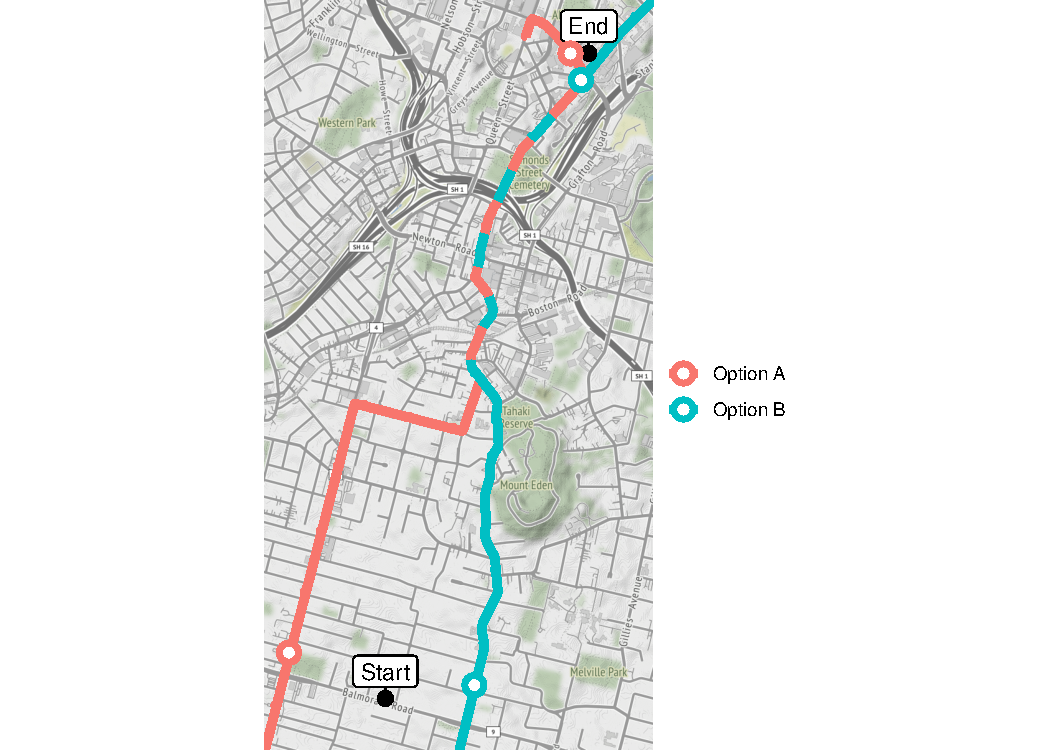
\includegraphics[width=\textwidth]{figure/eta_journey_arrival_prep-1} 

}

\caption[Route options]{Route options}\label{fig:eta_journey_arrival_prep}
\end{figure}


\end{knitrout}

\subsection{Choosing between two alternative routes}
\label{sec:journey_simple}



In this scenario, a passenger lives within walking distance of two major roads, along which various routes travel into the central city, as displayed in \cref{fig:eta_journey_arrival_prep}. The passenger must decide which route option to take before leaving home for the city. Let's say they have an appointment in town at 9~am, so at 8:10~am, they look at the real-time app on their phone and must decide whether to walk to route option A or B. Factors that will influence their decision may include:
\begin{itemize}
\item How long will I have to wait until the next bus?
\item What is the probability I will arrive in time for the next bus? And how long until the next one?
\item What is the probability that I will arrive at my destination on-time? And how early will I be?
\item How long will I be on the bus?
\end{itemize}
We can answer these questions using the \glspl{cdf} of arrival time at the start and end stops and taking into account walking times.


\begin{knitrout}\small
\definecolor{shadecolor}{rgb}{0.969, 0.969, 0.969}\color{fgcolor}\begin{figure}

{\centering 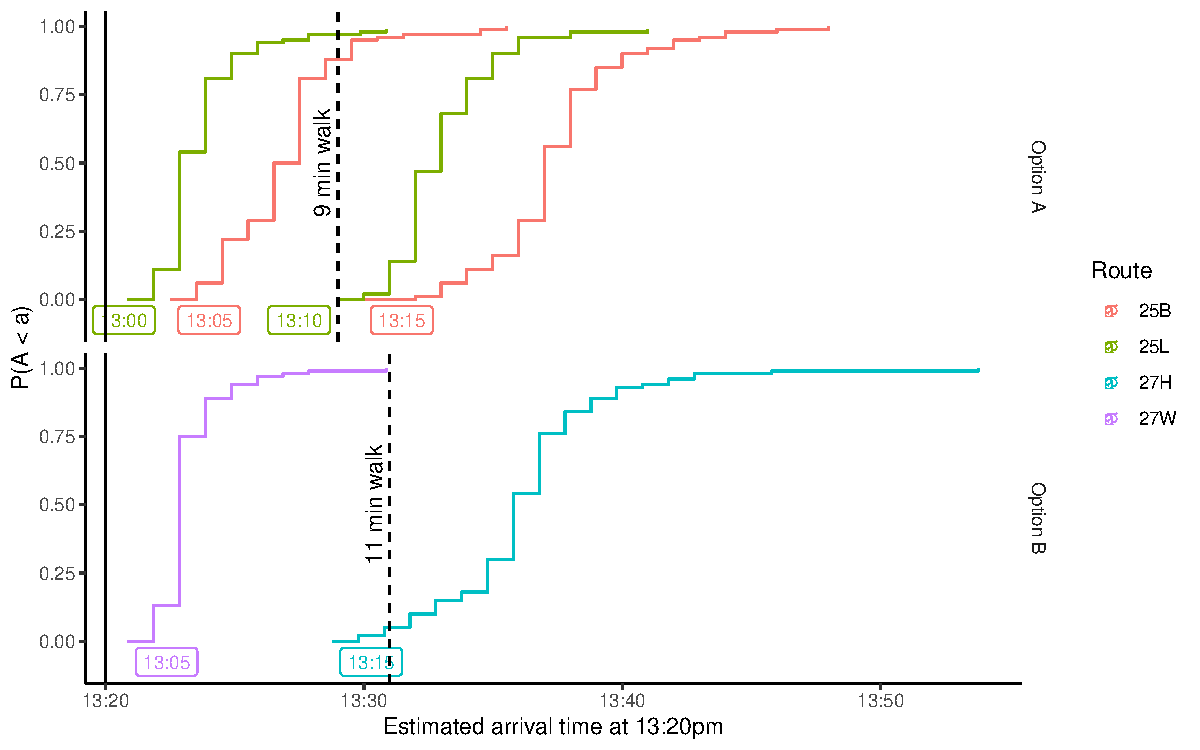
\includegraphics[width=\textwidth]{figure/eta_journey_arrival-1} 

}

\caption[ETA predictions for two route options]{ETA predictions for two route options. The coloured curves represent the CDF of arrival time for individual trips made at 7am. The vertical black lines indicate the estimated walking time (according to Google Maps) from the Start location to each stop.}\label{fig:eta_journey_arrival}
\end{figure}


\end{knitrout}


\Cref{fig:eta_journey_arrival} displays the \glspl{cdf} of all active trips\footnote{Our application currently only estimates arrival times for active trips.} along the two route options at 8:10~am when the passenger is about to leave home (solid line), and includes dashed lines representing the walking time to each of the alternative stops. At the lower end of each \gls{cdf} is a label indicating the trip's start time, which is the simplest method of identifying trips, and the curves are coloured by the route number. For option A, the passenger is likely to miss the 7:48 and 7:50 trips but has a 62\% chance of catching the 7:58. Additionally, two more active trips are arriving later, which the passenger could catch if they miss the 7:58. As for option B, the 7:45 trip is about to arrive at the stop, so can be ignored; if the passenger chooses this option, they have a 23\% and 99\% chance of catching the 7:56 and 8:05 trips, respectively. Since no further trips have begun, we cannot (yet) forecast how long until the next trip if they miss the 8:05 trip.



\begin{knitrout}\small
\definecolor{shadecolor}{rgb}{0.969, 0.969, 0.969}\color{fgcolor}\begin{figure}

{\centering 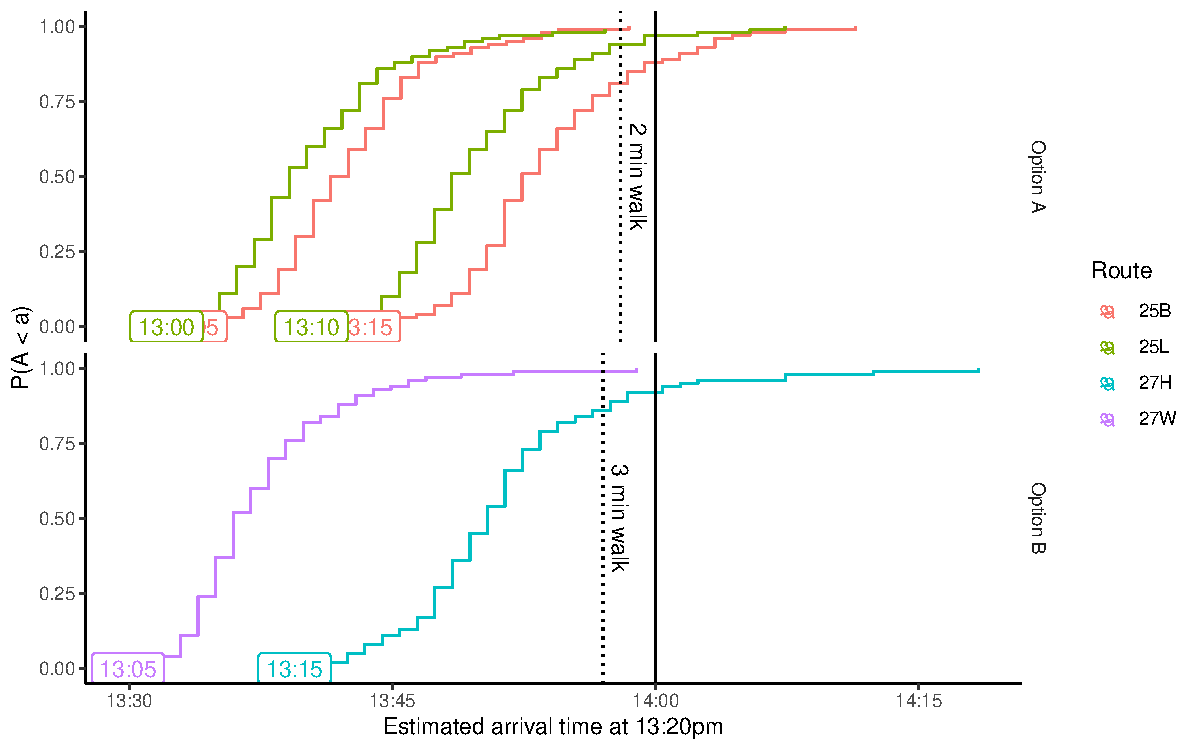
\includegraphics[width=\textwidth]{figure/eta_journey_arriveby-1} 

}

\caption[ETA predictions for two route options]{ETA predictions for two route options. The coloured curves represent the CDF of arrival time for individual trips made at 7am. The vertical black lines indicate the estimated walking time (according to Google Maps) from the Start location to each stop.}\label{fig:eta_journey_arriveby}
\end{figure}


\end{knitrout}

Based on the arrival results alone, it would likely make sense to walk to option A (a shorter walk) which has a decent chance of a short wait time; however, we also need to account for the passenger's appointment at 9~am. \Cref{fig:eta_journey_arriveby} provides \glspl{cdf} of the arrival time of the trips at the final stop, as well as vertical lines representing the appointment time (solid) and walking time (dotted). This time, we want the curve to be on the left-hand side of the dotted line, which is the case for most of the trips. For option A, the 7:58 has an (almost) 100\% chance of arriving on time, while the 8:00 and 8:08 have 98\% and 96\% chances, respectively. Option B tells a similar story, with (almost) 100\% for the 7:55 and 99\% for the 8:05 trips.


\begin{knitrout}\small
\definecolor{shadecolor}{rgb}{0.969, 0.969, 0.969}\color{fgcolor}\begin{table}

\caption{\label{tab:eta_journey_results}Journey planning.}
\centering
\fontsize{8}{10}\selectfont
\begin{tabular}[t]{lllrrllll}
\toprule
\multicolumn{1}{c}{} & \multicolumn{1}{c}{} & \multicolumn{1}{c}{} & \multicolumn{2}{c}{Particle filter} & \multicolumn{2}{c}{GTFS} & \multicolumn{2}{c}{Outcome} \\
\cmidrule(l{3pt}r{3pt}){4-5} \cmidrule(l{3pt}r{3pt}){6-7} \cmidrule(l{3pt}r{3pt}){8-9}
Option & Route & Trip & $P_\text{catch}$ & $P_\text{arrive}$ & Catch & Arrive & Catch & Arrive\\
\midrule
A & 25L & 13:00 & 0.02 & 0.99 & N & Y & N & Y\\
 & 25B & 13:05 & 0.05 & 0.99 & N & Y & N & Y\\
 & 25L & 13:10 & 0.98 & 0.94 & Y & Y & Y & Y\\
 & 25B & 13:15 & 1.00 & 0.81 & Y & N & Y & Y\\
\midrule
B & 27W & 13:05 & 0.00 & 0.99 & N & Y & N & Y\\
 & 27H & 13:15 & 0.90 & 0.86 & Y & Y & Y & Y\\
\bottomrule
\end{tabular}
\end{table}


\end{knitrout}


The values, along with the binary GTFS predictions\footnote{``yes, you will make it'' or ``no, you will not''} and the observed result\footnote{This is historical data, after all} are displayed in \cref{tab:eta_journey_results}. For our predictions, the capture probabilities are all valid, while the arrival probabilities are overly optimistic: the 8:08 on option A and 8:05 on option B have probabilities over 95\%, but the bus does not arrive in time. The GTFS-predictor correctly identified the tardiness of the 8:08 trip, but was not so lucky with the 8:05, which could indicate that this bus was somewhat later than usual.

It is worth noting at this point that, as mentioned in the previous chapter, the current state of our application leads to \emph{underestimates} of arrival time, so it would be wise to be cautious with decisions made based on the above probabilities. Future work improving the underlying speed model and restricting speeds more strongly could improve performance.




\begin{knitrout}\small
\definecolor{shadecolor}{rgb}{0.969, 0.969, 0.969}\color{fgcolor}\begin{figure}

{\centering 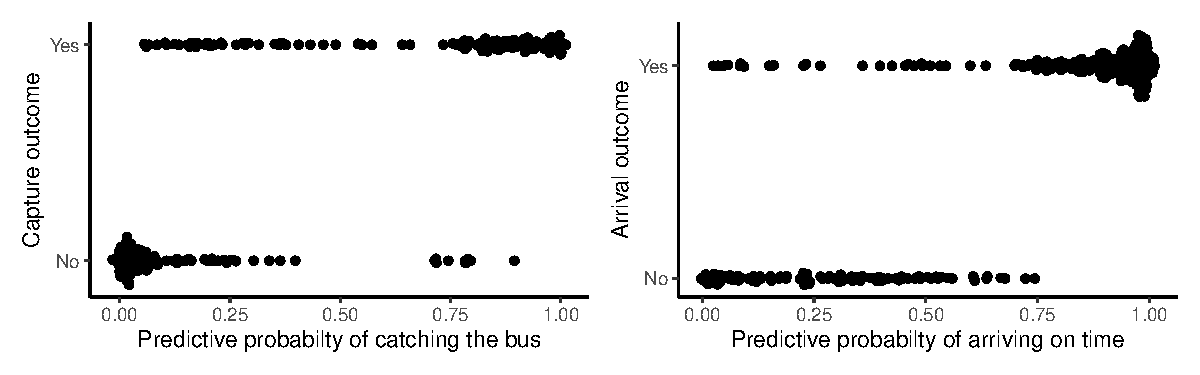
\includegraphics[width=\textwidth]{figure/eta_journey_results_avg-1} 

}

\caption[Results of performing the same journey planning prediction with different starting times (from 6am to 6pm), using the same start and end locations]{Results of performing the same journey planning prediction with different starting times (from 6am to 6pm), using the same start and end locations. Observations are whether or not the passenger would have arrived at the stop before the bus, jittered to better see each observation. The smoothed curve represents the mean, and indicates that on average our method is good at determining if the bus can be caught or not. Additionally, predictive probabilities of 0 and 1 have been removed.}\label{fig:eta_journey_results_avg}
\end{figure}

\begin{table}

\caption{\label{tab:eta_journey_results_avg}GTFS prediction results over all journeys, with the displayed values representing the proportion of outcomes in each cell (rows are conditioned by the GTFS prediction of Yes of No. }
\centering
\fontsize{8}{10}\selectfont
\begin{tabular}[t]{llllll}
\toprule
\multicolumn{1}{c}{} & \multicolumn{5}{c}{Observed outcome} \\
\cmidrule(l{3pt}r{3pt}){2-6}
\multicolumn{1}{c}{ } & \multicolumn{2}{c}{Catch bus} & \multicolumn{1}{c}{} & \multicolumn{2}{c}{Arrive on time} \\
\cmidrule(l{3pt}r{3pt}){2-3} \cmidrule(l{3pt}r{3pt}){5-6}
GTS Prediction & No & Yes &  & No & Yes\\
\midrule
No & 0.97 & 0.03 &  & 0.57 & 0.43\\
Yes & 0.11 & 0.89 &  & 0.01 & 0.99\\
\bottomrule
\end{tabular}
\end{table}


\end{knitrout}

Of course, the results in \cref{fig:eta_journey_arrival,fig:eta_journey_arriveby} and \cref{tab:eta_journey_results} are based on \emph{one single forecast} made at 8:10~am. To evaluate the performance of our prediction method, we repeated the process described above in 5~minute intervals between 6~am and 6~pm. For the appointment time, we used 15~minute intervals allowing for 30--45 minutes for the journey. That is, leaving between 7:15 and 7:30 had a targetted arrival time of 8~am; 7:30--7:45 targetted 8:15; and so on. In each case, we computed the probabilities for each of catching the bus and arriving on time. In \cref{fig:eta_journey_results_avg}, we have graphed the distribution of predicted probabilities for each of the two outcomes, for both catching the bus and arriving on time (A and B, respectively).

Further, \cref{tab:eta_journey_results_avg} presents a two-way contingency table for the binary GTFS predictions, with the outcome in rows. In 89\% of cases, the GTFS method correctly predicted that the passenger would catch the bus, and in 97\% of cases did it correctly identify that a passenger would miss the given trip. Conversely for the arrivals, in 99\% of cases the GTFS method correctly predicted that the bus would arrive on time; however, in only 57\% of cases did it correctly identify that the bus would \emph{not} arrive on time.


\subsection{Planning a multi-stage journey}
\label{sec:journey_transfer}

A more complex scenario is one where the passenger must transfer from one route onto another. Transfer journeys are common for travellers commuting from further afield, where there are often several \emph{feeder routes} which connect at a hub which usually has more frequent trips to another hub. It may also happen that your local route does not go to your destination, as is demonstrated in \cref{fig:eta_journey_arrival_prep}. In this scenario, the passenger must first catch a bus along route group A\footnote{We use route groups since there are several different routes which make the same journey, as can be seen with route group B in the south-west of \cref{fig:eta_journey_arrival_prep}.} to the stop marked ``Transfer'', at which point they disembark and wait for the next bus along route group B to get to their final destination (marked ``End'').



\begin{knitrout}\small
\definecolor{shadecolor}{rgb}{0.969, 0.969, 0.969}\color{fgcolor}\begin{figure}

{\centering 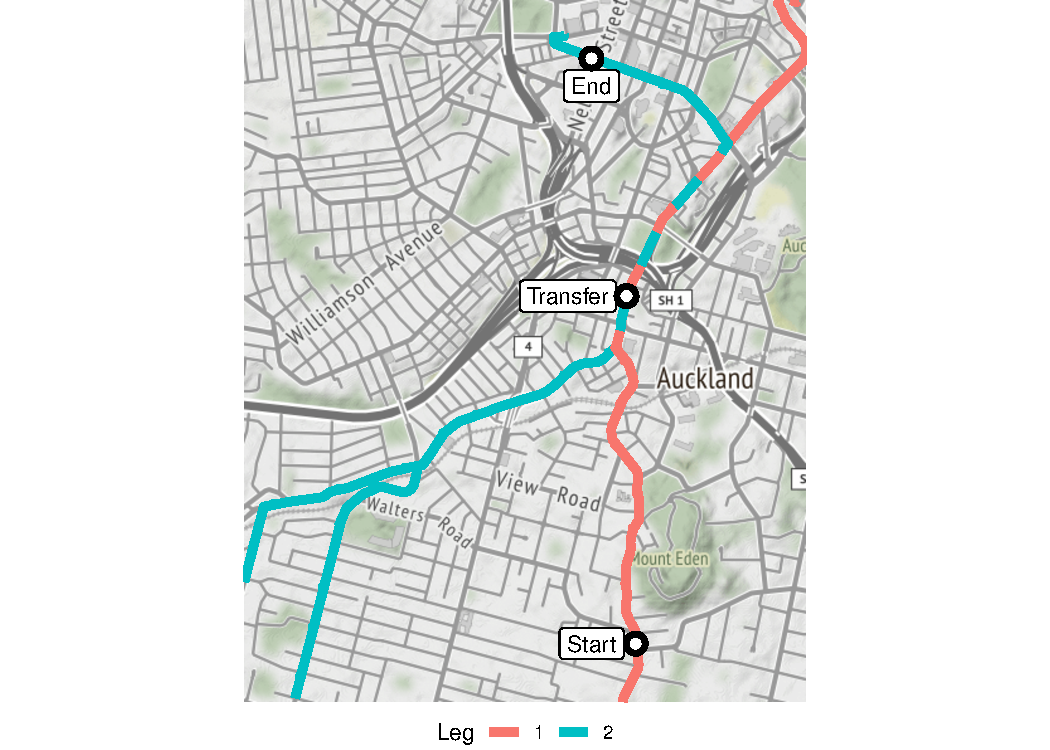
\includegraphics[width=\textwidth]{figure/eta_journey_transfer_prep-1} 

}

\caption[Transfer options]{Transfer options}\label{fig:eta_journey_transfer_prep}
\end{figure}


\end{knitrout}



\begin{knitrout}\small
\definecolor{shadecolor}{rgb}{0.969, 0.969, 0.969}\color{fgcolor}\begin{figure}

{\centering 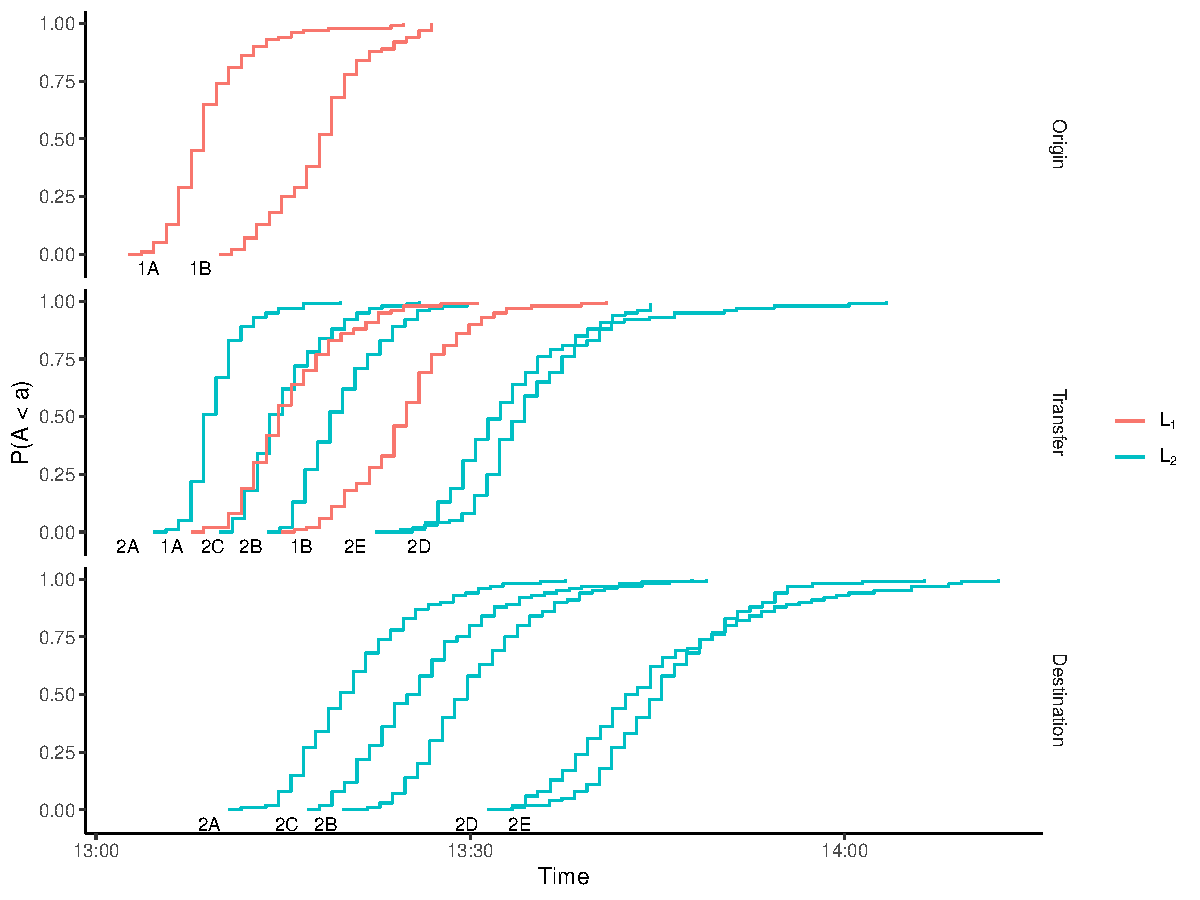
\includegraphics[width=\textwidth]{figure/eta_journey_transfer_graph-1} 

}

\caption[Arrival times]{Arrival times}\label{fig:eta_journey_transfer_graph}
\end{figure}


\end{knitrout}


Similarly to the previous example, we take one single forecast of all trip arrivals at 1~pm to make decisions. For simplicity, we leave out walking time, but as in the previous section this could easily be included, if desired. \Cref{fig:eta_journey_transfer_graph} shows, for all active trips at 1~pm, their arrival time \glspl{cdf} at the start and transfer stops (for the first leg) and the transfer and end stops (for the second). We could of course add additional constraints, such as arrival by a specific time, but in this instance we are solely intereste in whether or not each trip in group A will arrive \emph{before} the trips in group B.


To calculate the probability that a given trip along route A will arrive at the transfer stop before a given trip along route B, we use the following inequality:
\begin{equation}
\label{eq:eta_total_prob}
\begin{split}
\Pcatch =
\Pr{A < B} &= \sum_{x=1}^{\infty} \Pr{A < B\,|\,B = x}\Pr{B=x} \\
  &= \sum_{x=1}^\infty
    \Pr{A < x} \Pr{B=x} \\
  &= \sum_{x=1}^\infty
    \Pr{A < x} \left[
      \Pr{B < x + 1} - \Pr{B < x}
    \right]
\end{split}
\end{equation}
which we can easily compute given the \glspl{cdf} of the arrival time of each trip obtained from \cref{eq:pf_cdf_arrivaltime}. In table \cref{tab:eta_journey_transfer_res} we display the results, along with the binary predictions using GTFS and the observed outcomes. Our results appear reasonable at predicting transfer probabilities; in contrast, the GTFS makes one poor choice between A1 and B3, which it predicts \emph{will} connect, but infact they do not (our prediction was for a 32\% chance). This is where a prediction probability shows its power, in that a passenger could, where applicable, base their decision on how important it is they make the transfer. While this is a fairly non-exciting example (it's a short wait for the next bus), there are other situations where the headway between trips is 30--60~minutes, in which case missing a transfer by a few minutes would be frustrating. However, until our application has been updated to make predictions for upcoming (and not just active) trips, we could not obtain any examples of this.


\begin{knitrout}\small
\definecolor{shadecolor}{rgb}{0.969, 0.969, 0.969}\color{fgcolor}\begin{table}

\caption{\label{tab:eta_journey_transfer_res}Transfer probabilities}
\centering
\fontsize{8}{10}\selectfont
\begin{tabular}[t]{llrll}
\toprule
Leg 1 & Leg 2 & $\mathbb{P}_\text{transfer} & GTFS & Outcome\\
\midrule
1A & 2A & 0.04 & N & N\\
 & 2B & 0.71 & Y & Y\\
 & 2C & 0.32 & Y & N\\
 & 2D & 1.00 & Y & Y\\
 & 2E & 0.99 & Y & Y\\
\midrule
1B & 2A & 0.00 & N & N\\
 & 2B & 0.20 & N & N\\
 & 2C & 0.05 & N & N\\
 & 2D & 0.96 & Y & Y\\
 & 2E & 0.93 & Y & Y\\
\bottomrule
\end{tabular}
\end{table}


\end{knitrout}


As before, we proceed to repeat the procedure for multiple times (this time between 6~am and 8~pm), and compute the probabilities of available transfers and whether or not they connected. \Cref{fig:eta_journey_transfer_many} shows the predicted transfer probabilities grouped by outcome, and coloured by the GTFS prediction. This is complimented with contingency \cref{tab:eta_journey_transfer_many,tab:eta_journey_transfer_many2} for the GTFS method and our own, respectively. For the GTFS method, in 16\% of cases a predicted successfull connection failed, versus only 8\% using our method and a rule of $\Ptransfer > 0.5$. The false negative rate was similar for both methods, although slightly higher for our own (7\% versus 3\% for GTFS).


\begin{knitrout}\small
\definecolor{shadecolor}{rgb}{0.969, 0.969, 0.969}\color{fgcolor}\begin{figure}

{\centering 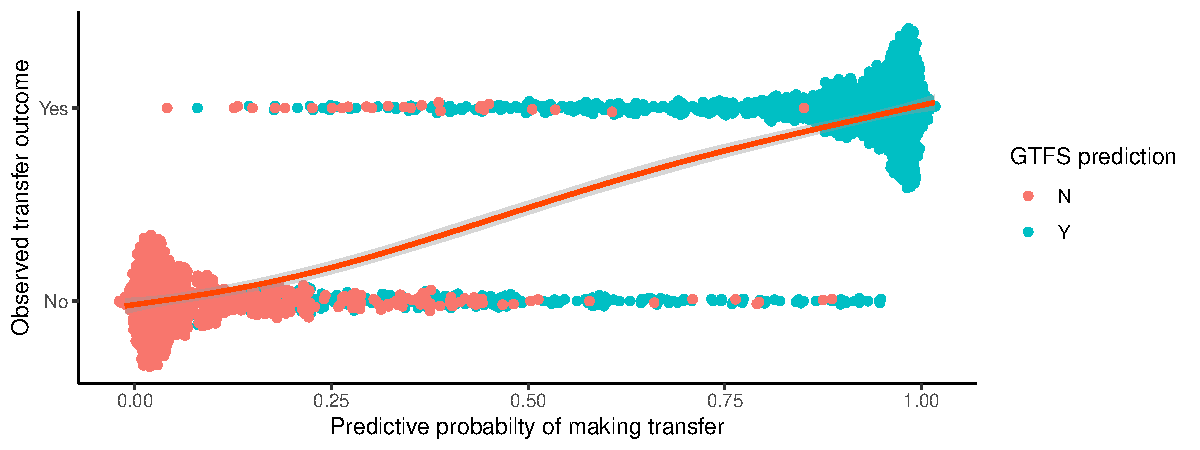
\includegraphics[width=\textwidth]{figure/eta_journey_transfer_many-1} 

}

\caption[Results of performing the same transfer journey planning prediction with different starting times (from 6am to 8pm)]{Results of performing the same transfer journey planning prediction with different starting times (from 6am to 8pm). Observations are whether or not the first bus would arrive at the transfer stop before the second bus, jittered to better see each observation. The smoothed curve represents the mean, and indicates that on average our method is good at determining if the bus can be caught or not. Additionally, predictive probabilities of 0 and 1 have been removed since, after checking, none or these were invalid and only served to distort the figure.}\label{fig:eta_journey_transfer_many}
\end{figure}


\end{knitrout}

\begin{knitrout}\small
\definecolor{shadecolor}{rgb}{0.969, 0.969, 0.969}\color{fgcolor}\begin{table}

\caption{\label{tab:eta_journey_transfer_many2}Results of running the transfer prediction problem over the course of the day. Rows represent the predicted outcome (No, the transfer will be made, or Yes, it will) and the numbers represent the proportion of predictions with each observed outcome. The GTFS rule is binary, while the particle filter results are based on transfer probability of at least 0.5, 0.8, or 0.95 (as indicated).}
\centering
\fontsize{8}{10}\selectfont
\begin{tabular}[t]{llllllllllll}
\toprule
\multicolumn{1}{c}{} & \multicolumn{11}{c}{Outcome} \\
\cmidrule(l{3pt}r{3pt}){2-12}
\multicolumn{1}{c}{} & \multicolumn{2}{c}{GTFS} & \multicolumn{1}{c}{} & \multicolumn{2}{c}{PF (P > 0.5)} & \multicolumn{1}{c}{} & \multicolumn{2}{c}{PF (P > 0.8)} & \multicolumn{1}{c}{} & \multicolumn{2}{c}{PF (P > 0.95)} \\
\cmidrule(l{3pt}r{3pt}){2-3} \cmidrule(l{3pt}r{3pt}){5-6} \cmidrule(l{3pt}r{3pt}){8-9} \cmidrule(l{3pt}r{3pt}){11-12}
Prediction & No & Yes &  & No & Yes &  & No & Yes &  & No & Yes\\
\midrule
No & 0.97 & 0.03 &  & 0.93 & 0.07 &  & 0.84 & 0.16 &  & 0.7 & 0.3\\
Yes & 0.16 & 0.84 &  & 0.08 & 0.92 &  & 0.03 & 0.97 &  & 0 & 1\\
\bottomrule
\end{tabular}
\end{table}


\end{knitrout}



In this section we have seen how having access to the full distribution of arrival times allows us to compute the probabilities of events, rather than make singular binary predictions of their outcome. This can enable more sophisticated decision making by travellers depending on their own needs. Of course, all of the examples shown were manually estimated, so some work is needed before it can be automatic, but the availability of the \glspl{cdf} for each trip and stop makes this easy. It has the additional advantage that, were any improvements to the vehicle or network models made, these would automatically be integrated into the arrival prediction component and immediately be used to adjust the probabilities. From here, it is up to travellers themselves, or other intermediate agencies (which could be a transport planning app, for example) to use the available information to make decisions.

\begin{itemize}
\item references on dynamic routing (it's a hard problem, etc etc)
\end{itemize}
